\documentclass[11pt]{article}

%	packages
\usepackage{amsmath}
\usepackage{amssymb} 
\usepackage{caption}
\usepackage{graphicx}
\usepackage{authblk}
\usepackage[hypertexnames=false,colorlinks=true,linkcolor=blue,citecolor=blue]{hyperref}
\usepackage[numbers,comma,square,sort&compress]{natbib}
\usepackage[a4paper,text={6.5in,10in},centering]{geometry}
\usepackage[caption=false]{subfig}
\usepackage{tikz}
\usepackage{enumerate}

%	layout
\setlength{\parindent}{0.0in}
\setlength{\parskip}{1.0ex plus0.2ex minus0.2ex}
\renewcommand{\baselinestretch}{1.2}

%	figures
\graphicspath{{./figs/}}

%\setcaptionmargin{0.25in}
\def\captionfont{\itshape\small}
\def\captionlabelfont{\upshape\small}

%	counters
\makeatletter\@addtoreset{equation}{section}\makeatother
\renewcommand{\theequation}{\arabic{section}.\arabic{equation}}

\newenvironment{Acknowledgment}%
 {\begin{trivlist}\item[]\textbf{Acknowledgments.}}{\end{trivlist}}

\def\Fix{\mathop\mathrm{Fix}\nolimits}

\newcommand{\R}{\mathbb{R}}
\newcommand{\C}{\mathbb{C}}
\newcommand{\N}{\mathbb{N}}
\newcommand{\Z}{\mathbb{Z}}

\def\Re{\mathop{\mathrm{Re}}}
\def\Im{\mathop{\mathrm{Im}}}

\newcommand{\rmO}{\mathrm{O}}
\newcommand{\rmo}{\mathrm{o}}
\newcommand{\rmd}{\mathrm{d}}
\newcommand{\rme}{\mathrm{e}}
\newcommand{\rmi}{\mathrm{i}}
\newcommand{\im}{\mathrm{Im}\,}
\renewcommand{\ker}{\mathrm{Ker}\,}
\newcommand{\id}{\mathrm{\,id}\,}
\newcommand{\ad}{\mathrm{ad}}
\newcommand{\Rg}{\mathrm{Rg}}


\begin{document}

\title{A Systematic Study of Altruism via Equation-free Methods}

\author{Spencer A. Thomas, David J. B. Lloyd, Anne C. Skeldon}
\affil{\small Department of Mathematics, University of Surrey, Guildford, GU2 7XH, UK}
\date{}
\maketitle

\renewcommand{\vec}[1]{\mathbf{#1}}


\begin{abstract}
%Analysis of the Altruism model using macroscopic techniques via equation-free bifurcation analysis. 
%
%systematic analysis reveals: small band of bi-stability with no stable mixed state, tipping points, large stable selfish domain, altruists stable in tough conditions. 
%
%dynamics are Gaussian in general (except D=0, H=0 where there are Dirac functions. Even Gaussian near the tipping point and shows an increase in variance as you approach the tipping point
%-> what about the other regime shifts?\\

{\bf DO LAST}
The emergence of altruism as an abstract trait is poorly understood. Despite many years of investigation, factors identified as drivers of the emergence of altruism are problem specific. The systematic analysis of a simple abstract model of altruisms may solve this problem, however to date none are available. Here we investigate a problem-independent agent-based model (ABM) of altruism using equation-free methods. This powerful techniques enables the macroscopic behaviour of ABMs to be mathematical modelled without any knowledge of the underlying dynamics of the system. Here we provide a systematic analysis of a model of altruism and how group dynamics are effected environmental conditions. Furthermore, we also provide a map in parameter space of the system dynamics, uncovering boundaries, bifurcations, transitions and tipping points in the model. Our results indicate that, in the absence of environmental pressures competition arises, and altruism only emerges when conditions become to hostile for individuals to survive alone. 

\end{abstract}


\section{Introduction}
\label{sec:intro}
{\bf needs citations and extra detail}
%Agent-based models (ABMs) 
%consist of individual entities (agents) which move and
%interact with each other according to a 
%defined set of rules. They are increasingly used to model complex
%systems where it is difficult to write down an explicit system-level 
%description of macroscopic behaviour and have been used in a 
%wide range of disciplines such as social science  and 
%psychology \cite{Li2008, Hughes2012}, 
%mathematics and network theory \cite{Lima2009}, policy 
%making and 
%economics \cite{Epstein2006,Gilbert2010,Feng2012}, 
%computer science \cite{Niazi2009, Niazi2011, Sarker2010} 
%and biology \cite{An2009, Barnes2010, Tang2007}.
%Their increasing use has spawned a number of software packages specifically
%designed for the non-mathematician/computer scientist to be able to 
%construct their own ABM, for example SWARM \cite{swarm} and Netlogo \cite{Netlogo}.
%
%One significant challenge with ABMs is developing a systematic
%understanding of their behaviour.  ABM's are typically stochastic in nature
%as a result of probabilistic interaction rules. 
%Consequently, model behaviour is usually
%understood through the use of Monte Carlo simulations. 
%Given the large number of parameters that
%are frequently embedded in the rules within an ABM, this approach 
%can be time-consuming.
%The fact that the interaction rules 
%at the microscopic (agent) level often lead to 
%macroscopic (emergent) behaviour of the system as a whole, suggests
%that %the use of stochastic numerical continuation methods is worthwhile.
%an alternative way to establish systematic ABM behaviour is with the
%use of parameter path-following techniques.

The emergence of collective behaviour in group dynamics has been studied in a wide range of disciplines including social \cite{Nowak1998}, mathematical \cite{Camerer2003} and biological \cite{Szathmary1999} sciences. The phenomenon of individuals working together within a collective is of particular interest has been studied in many system, from human tribes \cite{}, to small insects \cite{}, and in bacterial colonies \cite{}. Specifically, the development of altruism \cite{Boyd2003,Mohtashemi2003} is a well studies problem in social science \cite{Nowak1998,Janssen2014,Pepper2007}, game theory \cite{Camerer2003} and biology \cite{Szathmary1999}. However, the emergence of cooperative behaviour has been attributed to several factors: survival, enforcement, pay-off enhancement, cultural pressures, sustainability and prevention war. In many cases the solution to the altruism problem is in context of the system under investigation, indicating a lack of consensus for the causation of altruism in general. A systematic study of altruism, in an abstract system, is lacking \cite{Thomas2016ember}. In particular, questions regarding the conditions for altruism to arise still remain open. In this paper we use equation-free framework \cite{Theodoropoulos2000} to extract the macroscopic behaviour of an abstract agent-based model of altruism \cite{Mittleldorf2000}. Through this analysis we investigate under what conditions altruism, and other behaviours, arise, and identify the transitions between different macroscopic dynamics within the model. 


 

\section{Agent-based Models}
\label{sec:abm}

Agent-based models (ABMs) are extremely useful for simulating the dynamics of complex systems in the absence of a mathematical description of the systems dynamical behaviour. It is possible to simulate the dynamics of these highly non-linear systems by defining the interactions on the level of individual agents. The use of probabilistic rules enable the individuals to make `decisions' and ultimately give rise to stochastic dynamics at the system level. 

Although ABMs have been used in a wide range of disciplines to simulate the behaviour of complex systems in this way, their analysis is not straight forward. The non-linear interactions and (generally) stochastic nature obfuscate the effects of the model parameters and limit the insight that can be obtained by direct simulation. As a consequence most investigations run several configurations of parameters and aggregate the outcomes usually under the assumptions of Gaussian behaviour. These simplistic methodologies can obscure behaviours typically associated with complex systems, such as multiple stability; tipping points; regime shifts (e.g. bifurcations); and path dependency. 


\section{Equation-free Techniques}
\label{sec:ef}
Equation-free methods \cite{Theodoropoulos2000} have emerged as an extremely powerful technique in system level analysis over the last 15 years. In particular, the ability of equation-free techniques has enabled the numerical analysis of the macroscopic behaviour of systems that do not have closed form solutions. Additionally, this framework has also enabled the continuation of stochastic systems \cite{Barkley2006} and ABMs \cite{Thomas2016limno}. By circumventing the requirement of a closed form, or deterministic, equation, it is now possible to apply numerical continuation and bifurcation analysis directly to (more readily available) microscopic equations or simulations. 

Continuation (path following) and bifurcation analysis are well established mathematical techniques for the analysis of non-linear systems \cite{Doedel1991,Seydel1987}. These methods focus on obtaining stationary
(or periodic) solutions for fixed point problems. In this article we only consider stationary solution determined by solving  
\begin{equation}
\tilde x = f(\tilde x, \lambda),
\label{eq:steady}
\end{equation}
for $\tilde x$ at a given $\lambda$. Solutions are obtained by phasing Eq.~(\ref{eq:steady}) as a root finding problem,
\begin{equation}
f(\tilde x_i;\lambda_i)-\tilde x_i=0~.
\label{eq:fixed}
\end{equation}
For the initial problem at $i<2$ a guess can be made and a root finding method, solutions can be calculated using a damped Newton-Raphson. The first step $x_0$ is  solved for a given $\lambda$, then $x_1$ is solved by taking a small step in $\lambda$, $\delta\lambda$, and repeating the damped Newton-Rhapson method. 
Once at least two solutions are obtained, secant-based or least squares predictors can be used to predict solutions to Eq.~(\ref{eq:fixed}) at successive $\delta\lambda$ steps in $\lambda$ \cite{Thomas2016ember}. For sufficiently small $\delta\lambda$, the predictions are close to the solution of Eq.~(\ref{eq:fixed})  and can be obtained in a few iterations of a root finding method. This method of `continuing' along the solution branches is much more efficient than solving Eq.~(\ref{eq:fixed}) directly at each $\lambda$ or via simulation \cite{Thomas2016limno}. 

Numerical continuation methods are traditionally applied to deterministic systems, with an equation describing its macroscopic behaviour. However, continuation of stochastic systems, or those without closed form macroscopic equations, can be achieved by replacing the equation governing the macroscopic behaviour with a collection of appropriately initialised microscopic simulations \cite{Kevrekidis2009}. The ethos here is to take the probability density function (PDF) of the microscopic simulations as a proxy for the macroscopic behaviour. Path following is achieved by numerical continuation of stationary statistics of this PDF which are obtained through the equation-free framework \cite{Barkley2006,Thomas2016ember}. For simplicity for the following example we will only consider the mean of the PDF, though this is readily extendible to high order moments of the systems PDF \cite{Barkley2006}. Taking an ensemble of realisations of Eq.~(\ref{eq:fixed}) results in a PDF, with an corresponding mean, $\tilde X_i$. We can use $\tilde X_i$ (and higher order moments) as a proxy for the (unknown) macroscopic distribution $F(\tilde X_i,\lambda_i)$ by solving 
\begin{equation}
F(\tilde X_i,\lambda_i)+\bar{\epsilon}-\tilde X_i = 0,
\label{eq:ABM_PDF_samplingerror}
\end{equation}
where $\bar{\epsilon}$ is an error due to the finite sample size of the ensemble. 

\begin{figure}
\centering
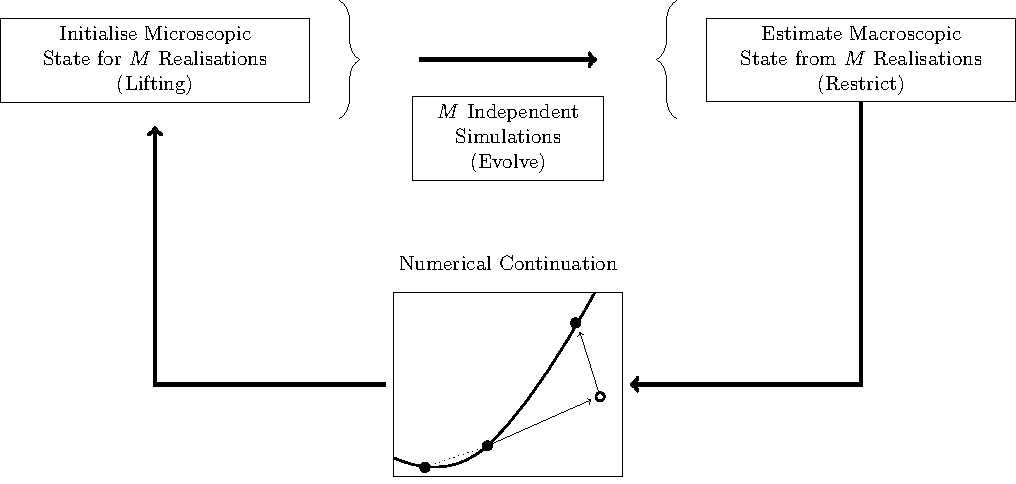
\includegraphics[width=0.8\textwidth]{EquationFree}
\caption{Schematic diagram of the equation-free framework for numerical continuation. \label{fig:ef}}
\end{figure}

The underpinning of equation-free methods is that there is a separation of time-scales between the micro- and macro-scales. This separation causes the dynamics of the system be dominated by the slower low order moments rather than the fast higher order moments \cite{Kevrekidis2003}. The slow manifold of the system can be approximated by a few of these low order moments \cite{Kevrekidis2009}.
Previous investigations have used equation-free methods to analyse stochastic systems \cite{Barkley2006}, biological models \cite{Erban2007}, chemical systems \cite{Kevrekidis2003}, fluid mechanics \cite{Li2007}, social systems \cite{Thomas2016limno}, experimental setups \cite{Sieber2008} and ABMs \cite{Avitabile2014, Thomas2016ember}.


%Although successful at simulation complex behaviour in the absence of a mathematical form of the macroscopic behaviour, such as partial differential equation, the rule based nature of ABMs causes limitations in the their analysis. Typically simulations are often average of some large number of runs, or analysed using parameter sweeps. This raises several issues; 1) systems are often assumed to be normally distributed; 2) the level of noise in the system is not often controllable or known {\em a prior}; 3) is only able to analysis stable states; 4) provides no information about the transient behaviour of the system; 5) time simulations are often time consuming. Moreover, in many cases the tools that perform the batch analysis does not analyse the output, thus this must be done manually in third party software packages. 

%The development of equation-free techniques \cite{Theodoropoulos2000} enable the application of well established analytical methods, which traditionally require an equation of state, to models with no mathematical description. These techniques provide a platform for detailed analysis of the macroscopic dynamics of systems such as stability and bifurcation analysis. Identifying the dependencies and transitions in the system map out the dynamics and can locate interesting regions of behaviour. {\em list the benefits of EF and what it can do}.

%Specifically, equation-free techniques allow the use of well established continuation and bifurcation methods to analyse a systems dynamic behaviour.  
%Essentially the need for a description of the systems macro-level dynamics is replaced with an ensemble of appropriately initialised micro-level simulations. 
The generalised framework involves a three step process; 1) initialising the micro-level system from the macro-level ({\em Lifting}); 2) running the simulation forward in time ({\em Evolving}); and 3) estimating the macro-level state from the ensemble of micro-level simulations ({\em Restricting}). The use of a root-finding algorithm and parameter step processes between the {\em Lift} and {\em Restrict} operators extend this framework to continuation of the macro-level system based on the micro-level simulation. That is, the root-finding algorithm can obtain fixed points in the system by evaluating the difference between the {\em Lift} and {\em Restrict} operators. As with classical numerical continuation, this fixed point can be used to predict the stationary solution with a step in parameter space. Thus we can perform systematic analysis of the dynamics of a system. This includes tasks that are inappropriate for direct simulation only, such as the analysis of unstable states in the system. Moreover, continuation methods can be much more computationally efficient that repeatedly performing long time simulations under parameter variation \cite{Thomas2016ember}.

Equation-free techniques enable the application of continuation methods to stochastic systems and micro-level models to analyse the macro scale dynamics \cite{Kevrekidis2009}. As a result they have been successful in the system-level analysis of; stochastic systems \cite{Barkley2006} physical experiments \cite{Sieber2008,oscillations}, ABMs \cite{Avitabile2014, Thomas2016limno}, micro-level simulations \cite{Frederix2007,Frederix2009}. 

Agent-based models are stocahsitc in general and the, particularly in real world models, the level of noise is immutable. This can be particularly problematic for equation-free methods as they rely on extracting the macro-level behaviour from the distribution of realisations of the micro-level model in the {\em Restrict} step. Typically the only way to circumvent the level of noise is to increase the number of realisations to 100s of thousands, or even millions \cite{Barkley2006}. This can cause extremely long computational runtimes as a single time steps ABM can take 10s of seconds and may require a large number of time steps to converge to a fixed point, even when using an appropriate {\em Lift} operation where less time steps for convergence are required than direct simulations. Some techniques have been implemented to improve the robust of continuation of noisy systems \cite{}. Here we use the convergence constraint corrector repeat (C$^3$R) procedure as it has been shown to be extremely robust for continuation around folds at high levels of noise and at significantly reduced number of realisations \cite{Thomas2016ember}. The C$^3$R algorithm determines an acceptable bounds (constraint) for convergence of the corrector part of the equation-free continuation framework that are based on the statistics of the models dynamics. If outside of this bounds successive predictions are likely to be poor leading to a failure of the standard predictor corrector methods. Therefore, in the case of a converged solution falling outside of this constraint, the corrector procedure is re-initialised and repeated. This whole process is repeated a maximum of 10 times before the computation is abandoned to avoid repeated computation where a solution can not be found.

Bifurcation are detected through monitoring the sign of the determinant of the Jacobian as this has been used in a large number of implementations \cite{}. The Jacobian is determined thourgh finite differencing. Although matrix-free methods have been shown to be more robust than finite differencing, it requires more computation and as the Jacobian is required for the predictor-corrector method, this method of bifurcation detection come as little additional computational cost. Moreover, for simulators such as ABMs, a single time step in the model may take a reasonable amount of time so methods that reduce computation time, such as finite differencing and C$^3$R methods are favourable.


\section{A Model of Altruism}
\label{sec:model}

Agents exist at each site on a fixed size 2D lattice and can be altruistic ($A$), selfish ($S$) or empty ($E$). Empty agents represent a `dead' state but contributes to the systems dynamics as the other agent. The altruists agents share resources or benefits with their neighbours (regardless of neighbour type) at a cost to the altruistic individual. Selfish agents receive this shared benefit from any neighbouring altruists, but do not share any themselves and thus do not incur a cost.

At successive time intervals, the agents compete for occupation of a given lattice site in the next iteration. This is analogous to parents competing for their offspring to exist in the next generation cycle. The competition for a given location $(i,j)$ occurs between the current agent at $(i,j)$ and its four neighbours, the agents at locations $(i-1,j)$, $(i+1,j)$, $(i,j-1)$, and $(i,j+1)$. The lattice is wrapped around the boundaries so that there are no edge effects and the agents here interact with the agents at the opposite edge. The basis of this model is taken from \cite{Mittleldorf2000} and has been implemented as an ABM in the NetLogo library \cite{Altruism}.

In general the results of the ABM depend on the environmental conditions. However, for individual simulations, the state of the system can vary due to the probabilistic rules governing the competition between agents. Stochasticity is introduced through random spatial distributions of agents at the start of each simulation and contributes to the dynamics of the model. 

The probability of a given agent occupying a given lattice position in the next generation is based on the agents currently in the neighbourhood of the site at the current time step. The probability of an agent occupying position $(i,j)$ are given by $p_A, p_S$ or
$p_E$ for altruistic, selfish or empty agents respectively.
These probabilities are updated at each time step $n$ and are defined as

\begin{eqnarray}
p_{A_{i,j}}^{n+1} & = & \frac{F_{A_{i,j}}^n}{F_{T_{i,j}}^n} \label{eq:PA}\\
p_{S_{i,j}}^{n+1} & = & \frac{F_{S_{i,j}}^n}{F_{T_{i,j}}^n} \label{eq:PS}\\
p_{E_{i,j}}^{n+1} & = & \frac{F_{E_{i,j}}^n+D}{F_{T_{i,j}}^n} = 1-p_{A_{i,j}}^{n+1} - p_{S_{i,j}}^{n+1}~, \label{eq:PE}
\end{eqnarray}
where $F_{A_{i,j}}^n, F_{S_{i,j}}^n$ or $F_{E_{i,j}}^n$ represent the `fitness' of the agent at position $i,j$ for a given type. $F_A$ and $F_S$ represent agents of type altruist or selfish, and $F_E$ is the fitness of an empty state (the minimum fitness required to survive in the environment). The total fitness at position $(i,j)$, $F_{T_{i,j}}^n$, is based on the fitness of the neighbouring agents and is calculated as
\begin{eqnarray}
F_{A_{i,j}}^n & = & 1 - C + B\frac{N_{A_{i,j}}^n}{5}~, \label{eq:FA} \\
F_{S_{i,j}}^n & = & 1 + B\frac{N_{A_{i,j}}^n}{5} ~,\label{eq:FS} \\
F_{E_{i,j}}^n & = & H~. \label{eq:FE}
\end{eqnarray}
Here $N_{A_{i,j}}^n$ is the number of altruist agents in the neighbourhood of $(i,j)$. System parameters $B$ and $C$ correspond to the benefit shared by altruists and its associated cost to them respectively. Parameter $D$ represents a fixed death rate for all agents and $H$ is the harshness of the environment (the fitness of the dead state).
From Eq.~(\ref{eq:FA})-(\ref{eq:FE}) the total fitness can be determined as 
\begin{equation}
F_{T_{i,j}}^n = F_{A_{i,j}}^n + F_{S_{i,j}}^n + F_{E_{i,j}}^n + D~. 
\end{equation}

The fixed lattice size imposes a constraint on the total number of agents $N_T$ in the system. Therefore the relative number of each of the three agent types must sum to unity, $(N_A+N_S+N_E)/N_T=1$. This limits the possible states of the system in $f(N_A,N_S,N_E)$ space to a surface that adheres to the conservation of $N_T$. 

Due to Eq.~(\ref{eq:PA})-(\ref{eq:PE}) the probability of an agent existing in successive generations is dependent on that agent existing in the previous generation. Due to the overlapping neighbourhoods, it is possible that agents disappear and reappear on a local scale. 
However, over the entire lattice if an altruist or selfish agent is not present in a generation, then it can not exist in future generations. That is, there is no regeneration. The empty state is excluded from this restriction in the presence of a non-zero $D$ due to Eq.(\ref{eq:PE}) ensuring the probability is always non-zero.


\section{Results and Discussion}

In order to examine the macroscopic behaviour of the altruism model described in \S\ref{sec:model} we perform equation-free analysis as outlined in \S\ref{sec:ef}. Initially we investigate the dependence of the macroscopic behaviour of the altruism model on the disease parameter $D$ as this has been shown to be a bifurcation parameter in this model \cite{Thomas2016ember}.

To perform the computational analysis, we use the Emergent and Macroscopic Behavioural ExtRaction (EMBER) implementation introduced in \cite{Thomas2016ember}. The EMEBR algorithm has been applied to a real-world ABM and extracted bifurcations in the systems macroscopic behaviour and important drivers for the complex system \cite{Thomas2016limno}. This implementation also includes a {\em convergence constraint and corrector repeat} ($C^3R$) algorithm for numerical continuation that drastically improves robustness to noise whilst also significantly reducing the number of microscopic realisations for continuation \cite{Thomas2016ember}. Fewer microscopic realisations reduces the necessary computation time for the analysis, which for real world models becomes increasingly important as individual stimulations can take of the order hours to reach a stationary state.   




\subsection{Bifurcations in Disease}
\label{sec:disease}
Initially we consider the macroscopic state of this model as the $D$ is varied with the other parameter set as $B=0.48$, $C=0.13$, and $H$ = 1.0. The results of this analysis are given in Fig.~\ref{fig:SaddleNode}. Here we see that there are no solutions for the existence of the selfish agents under these conditions. In addition we observe a saddle node bifurcation occurs in the Altruism branch initially beginning stable until reaching the limit point at $(0.27,0.49)$. The limit point occurs as the stable branch collides with an usable branch that also exits in this region of $D$ which begins ar $(0,0)$ and extends to the limit point. There is also a bifurcation at $(0,0)$ where the unstable altruist branch collide with the unstable branch of the empty agents making it stable. At $D=0$ the empty branch is unstable as there is no death rate in the altruist agents thus the population $N_A \rightarrow N_T$. At $D<0$ death occurs in the altruists population thus the empty branch becomes stable and exists simultaneously with the stable altruist branch in Fig.~\ref{fig:SaddleNode}. The unstable altruist branch specificity the necessary initial population level in the altruism population in order to survive for a given $D$, $U_A(D)$. Noise in the system may cause some fluctuations on the individual level, however in general, if $N^0_A>U_A(D)$ the population is stable and will tend to the Fig.~\ref{fig:SaddleNode}. However, if $N^0_A<U_A(D)$, then the population is unsustainable and will die out as the system converges to the stable empty branch. Consequently there are two regimes in this state, a bi-stable regime between the altruist and empty agents, and a regime where only the empty agents survive. The boundary between these regimes, the limit point, corresponds to a catastrophic loss in the altruist population. As this model has no regeneration, once the altruists die out they can not be recovered, i.e. the path dependence is irreversible. Consequently there are two regimes in this state, a bi-stable regime where either altruists of empty agents survive dependent on initial number of altruistic agents (characterised by the unstable branch), and a regime where only the empty agents survive, a dead state. The boundary between these regimes, the limit point, corresponds to a catastrophic loss in the altruist population. As this model has no regeneration, once the altruists die out they can not be recovered, i.e. the path dependence is irreversible. 

\begin{figure}[h]
	\centering
	\includegraphics[width=0.8\linewidth]{SaddleNodeFull}	
	\caption{{\bf Saddle node bifurcation in the altruism model.} Stability is 
	indicated by solid (dashed) lines for stable (unstable). Model parameters are $B=0.48$, $C=0.13$ and $H=1.0$ with bifurcation points indicated by arrows. The distribution of the microscopic realisations at several locations along the branches are labelled. The probability density functions (PDFs) of the realisations are well characterised by Gaussian distributions, even close to the limit point as indicated with the blue curves. The variance of the PDFs are given for each continuation step. {\bf change ylabel in top left plot}
	}
	\label{fig:SaddleNode}
\end{figure} 

Under these conditions, there is a special case at $D=0$ as the system becomes deterministic. The lack of a solution for the selfish agents removes any competition for the altruists and without the death rate $D$ removing individuals the system will converge to one of two possible state dependent only on the initial number of altruists. As the empty branch is unstable and there is no regeneration, this state is only reached if and only if $N^0_A=0$. Any other initial state will lead to $N_A=N_T$. In either case, the PDF of microscopic realisations is a delta function with zero variance. At any other value of $D$ the system undergoes a bifurcation and becomes stochastic with $N_A<N_T$ with the PDF of realisations having a non-zero variance. In this regime the altruist PDF along both the stable and unstable branches are well characterised by Gaussian distributions, including near the limit point, as shown in Fig.~\ref{fig:SaddleNode}. The PDFs along the unstable branch have a higher variance compared to the stable branch due to the dynamics of the system tending to move it away from this fixed point. Therefore there are two variance curves corresponding to the two solution branches for the altruist agents. The variance of the PDFs along the stable and unstable branches increase with $D$ until a maximum value at the limit point, where both branches and variance curves meet as shown in Fig.~\ref{fig:SaddleNode}. The change in variance with $D$ implies that the Altruisms population, under these conditions, is Heteroscedastic. The observation of variance increasing until a maximum value at a limit point agrees with \cite{Ditlevsen2010} who used increasing variance alongside increasing autocorrelation, has been used as an indication of a regime shift or limit point. 

\begin{figure}[h]	
	\centering
	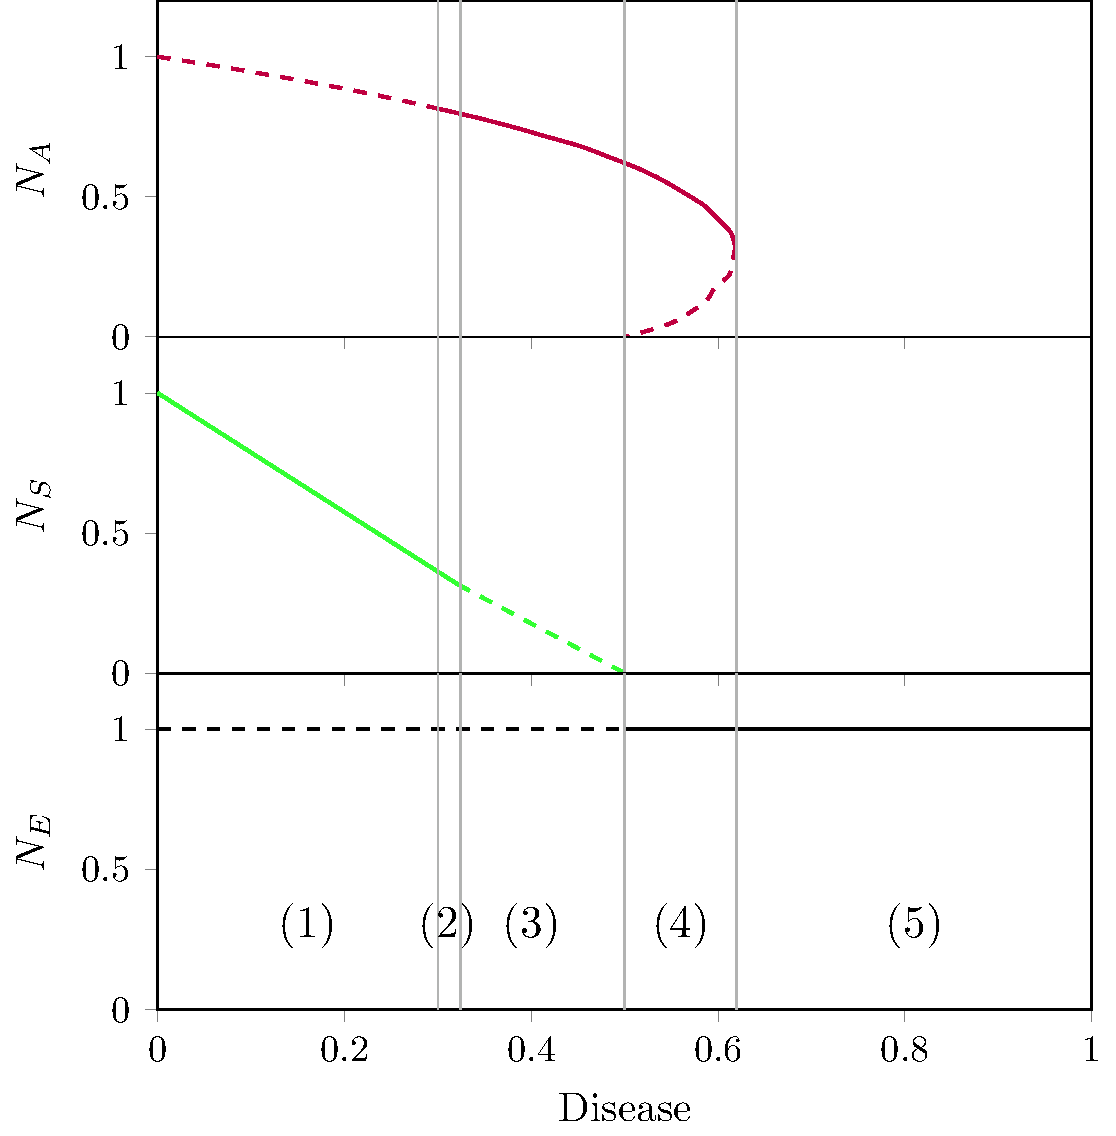
\includegraphics[width=0.8\linewidth]{AltruismD+H-D}	
	\caption{Bifurcation curve for the altruism model. Stability is 
	indicated by solid (dashed) lines for stable (unstable) branches 
	and vertical lines indicate regions of behaviour separated by bifurcation 
	points. Parameters: $C$ = 0.13, $B$ = 0.48, $H$ = 0.85.
	}
	\label{fig:altruistBifurcationD}
\end{figure}

Under similar parameter settings, with $H=0.85$, this system was shown to have a stable solution for the selfish agents \cite{Thomas2016ember}. We investigate the system under the same conditions as \cite{Thomas2016ember} where the bifurcation results are shown in Fig.~\ref{fig:altruistBifurcationD} it is clear that several bifurcations occur in this model under the variation of the disease parameter $D$. Bifurcations occur in the equilibrium branches of both Altruist and Selfish agents where when a new, unstable, path emerges connecting the two branches. This new branch connects the two agents in the plane of $F(N_A, N_S, N_E)$ space where the total number of agents is conserved. This branch corresponds to a state where both agents co-exist in the environment. However, this branch is highly unstable, inheriting the stability of the Altruist branch, and quickly collides with the stable Selfish branch causing it to be come unstable. The existence of this unstable state results in a narrow window of $D$ where a stable state exists for both agents, region 2 in Fig.~\ref{fig:altruistBifurcationD}. 
	

 

\subsection{Bifurcations in Harshness}
\label{sec:harshness}

%{\bf what about the variance of the alt / selfish branches when H=0.85? or when continuing in H?}


As stated in \S~\ref{sec:disease}, the shift from Fig.~\ref{fig:altruistBifurcationD} to Fig.~\ref{fig:SaddleNode}, as well as the disappearance of the Selfish branch, implies the system undergoes a global bifurcation between $H=0.85$ and $H=1.0$. The solution branch for the selfish agents vanish leaving a saddle-node in the altruist branch and a stable path for the empty state. We also perform numerical continuation of this parameter for a fixed $D$ with the results show Fig.~\ref{fig:altruistBifurcationD} with a fixed value of disease and varying the Harshness yields Fig.~\ref{fig:altruistBifurcationH}. Clearly the selfish agents depend non-linearly on the Harshness, unlike the Disease where the relationship is approximately linear. The non-zero Disease value means that even at $H=0$ neither strategy can sustain a full population under any state of the system. Compared to their dependence on $D$, both the altruists and selfish agents are not strongly dependent on $H$ below $H\approx0.4$ and both decrease approximately linearly. Above this value of however, both vary strongly with $H$ and again the altruistic branch experiences a limit point. The empty branch begins unstable and remains so until it coalesces with the second unstable path in the altruist, which emerges from the saddle-node bifurcation. The overall macroscopic behaviour with $H$ resembles that of $D$, each with five regimes caused by four bifurcation points. The bifurcation points in all agents and dependence of the selfish branch are different and further indicates that both $H$ and $D$ are bifurcation parameters. 
 
 
\begin{figure}[ht]
	\centering
	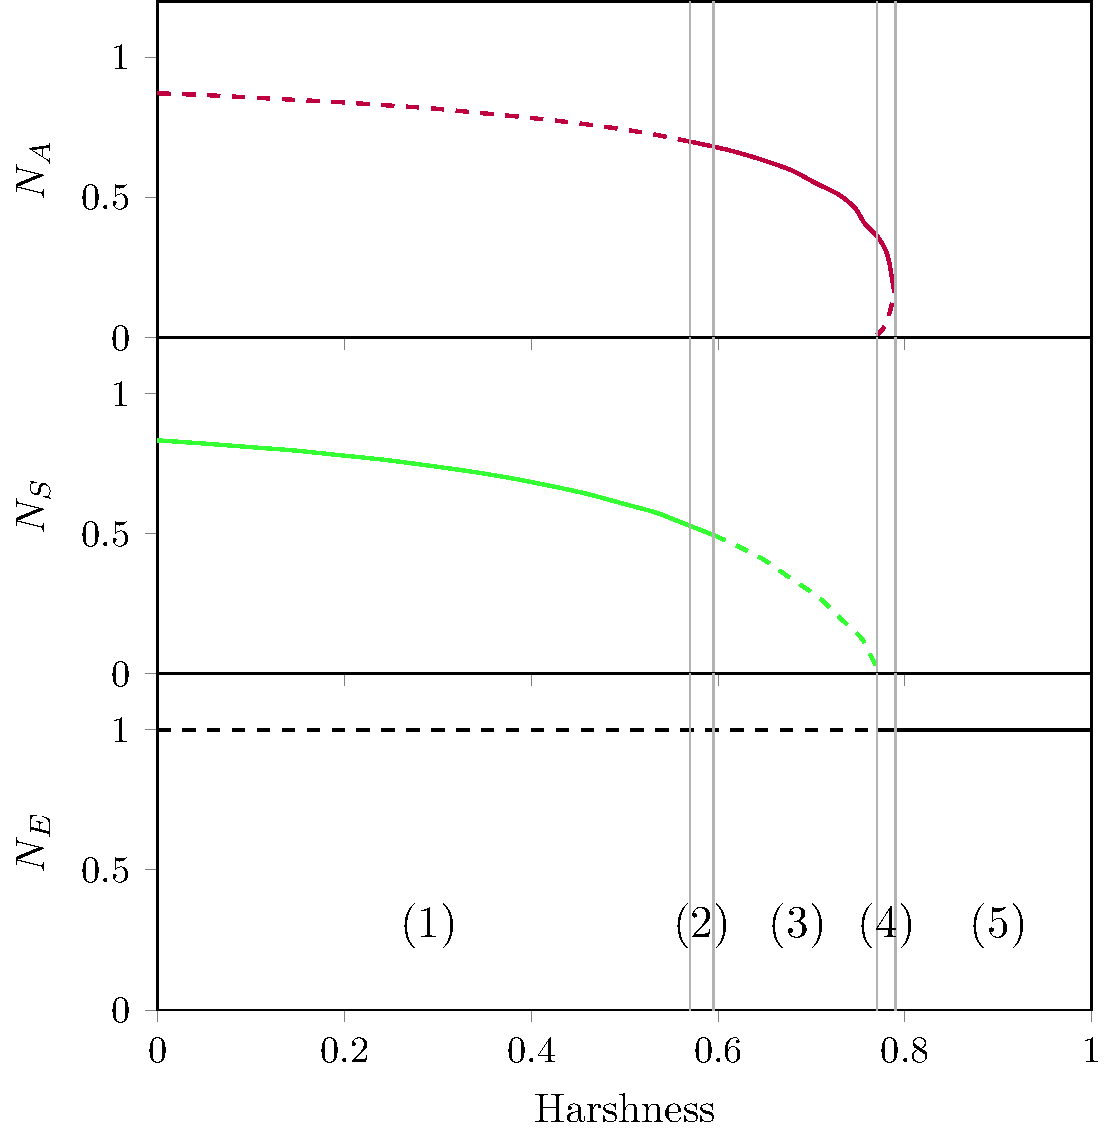
\includegraphics[width=0.8\linewidth]{AltruismD+H-H}	
	\caption{Bifurcation curve for the altruism model. Stability is 
	indicated by solid (dashed) lines for stable (unstable) branches 
	and vertical lines indicate regions of behaviour separated by bifurcation 
	points. Parameters: $C$ = 0.13, $B$ = 0.48, $D$ = 0.80.
	}
	\label{fig:altruistBifurcationH}
\end{figure}	



%Find a reference for biological system with irreiversible hystereis caused by the 2nd tipping point being in a infesible/impractical/unrealisitc region (eg negative quantity of something) and refer to the altruistic branch for low D where tipping point it at $H > 1$

\subsection{Bifurcations in 2D}


 \begin{figure}[h]
	\centering
	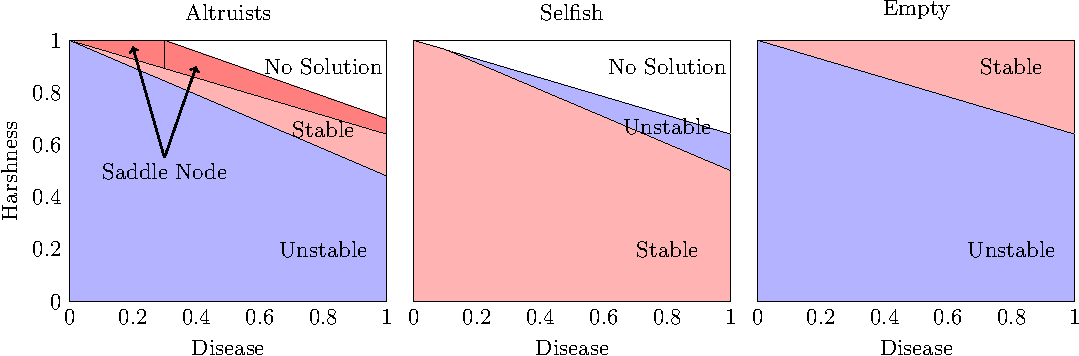
\includegraphics[width=0.8\linewidth]{2DBifurcationsAgents}	
	\caption{2D bifurcation diagrams for the players in the altruism model. Several bifurcations are observed indicated by the boundaries in each plot.  
	\label{fig:2Dagents}}
\end{figure}	


In order to analyse the macro-level dynamics of the altruism model under the variation of both the $D$ and $H$ parameters we conduct a series of equation-free numerical continuation experiments. Continuation for two or more parameters simultaneously is difficult, and estimations of bifurcation points is extremely challenging {\bf Kevrekidis paper?}. Therefore we perform continuation of each parameter independently with the other at fixed and repeat this for intervals of the fixed parameter. To ensure completeness, this process is repeated so that both $D$ and $H$ are analysed via the equation-free method. 

The results of the numerical studies are used to build a map of the systems stability and location of bifurcations. These maps are shown in Fig.~\ref{fig:2Dagents} for each agent and how this varies with environmental conditions. Clearly the selfish strategy is dominant for the majority of the parameter space. At low disease and harshness values it is not necessary for altruistic behaviour to support the group, thus the relative cost of altruism is too high and ultimately altruists are eliminated by the selfish agents. At low values of $D$ the selfish agents are stable and therefore dominate for all values of $H$ where a fixed point exists. As $D$ and $H$ increase, the conditions become more difficult there is a transition in the system where altruists can now survive and the selfish becomes unsustainable. At this point the benefits of being altruistic out weigh the relative costs. In even more difficult environments (top right of the plots in Fig.~\ref{fig:2Dagents}) we can see that there is no longer a fixed point for the selfish strategy. Here populations of selfish agents can not survive under any configuration. For the selfish agents $H\approx 0.5$ is a global bifurcation here below this value only stable solutions exist of all values of $D$, and conversely only unstable solutions exist for the altruism population. Above this threshold, for $D\neq0$, there exist unstable solutions, as well as a regime with no solution, for the selfish population. Increasing $D$ appears to increase the range of the unstable and no solution regimes while the extent of the stable branch decreases.

The altruistic population exhibits several types of bifurcation under the variation of both $D$ and $H$. In addition to the unstable, stable and no solution regimes that broadly correspond to the regimes in the selfish stability map, the altruist population also exhibits a saddle-node bifurcation. Interestingly the saddle-node observed in Fig.~\ref{fig:altruistBifurcationD} is present through all values of $D$. We do however divide this in to two distinct regions in Fig.~\ref{fig:2Dagents} as below $D\approx0.3$ the limit point is at $H>1$ and therefore no longer in the feasible region of this model. Despite the limit point exisiting in an infeasible regime, the stable and unstable branches of the saddle-node exist in the parameter space. Unlike the selfish population, which constantly reduces in size until it is becoming unstable or disappearing, the altruism population experiences an abrupt collapse at a limit point. This is represented by the boundary between the red (saddle node) and white (no solution) regions in Fig.~\ref{fig:2Dagents} of the altruists is at $N_A>0$. The emergence of the unstable altruist branch of the saddle-node is due to the collision of the unstable selfish branch with the unstable empty branch. At this point the selfish branch disappears causing the emergence of an unstable altruist branch and a stability change in the empty branch. The system now contains a stable branch for the altruists population and the empty state with an unstable altruistic populations state between them as shown in region $(4)$ of both Fig.~\ref{fig:altruistBifurcationD} and Fig.~\ref{fig:altruistBifurcationH}. 

Eventually, as the environment becomes increasingly hostile, even the altruists can not survive. This corresponds to the limit point in the altruist saddle-node where the stable and unstable branches collide and the solution for the altruistic population vanishes. Without either a altruist or selfish solutions, the only state in the system is a stable empty state which encompasses the rest of the parameter space. 



 \begin{figure}[ht]
	\centering
	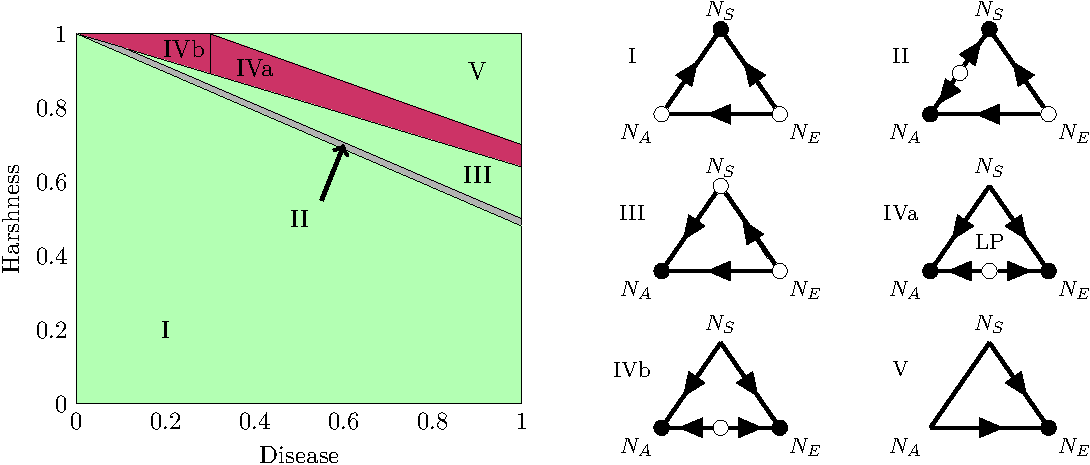
\includegraphics[width=0.8\linewidth]{2DBifurcationsSystem}	
	\caption{2D bifurcations for the system in the altruism model. (left) Several bifurcations are observed and labelled. Regions I, II and V (green) denote a single stable fixed point in the system, region II (grey) and region IV (purple) indicate the existence of a bistable system. (right) Phase diagrams of system dynamics in each region. The existence of a saddle-node is present in region IV, though the limit point in IVb is at $H>1$ therefore is distinguished from IV.
	\label{fig:2Dsystem}}
\end{figure}	

Combining the individual agent stability and bifurcation maps in Fig.~\ref{fig:2Dagents} provides insight into the system-level behaviour under the variation of $D$ and $H$, as shown in Fig.~\ref{fig:2Dsystem}. Here we can see the $(5)$ regions depicted in Fig.~\ref{fig:altruistBifurcationD} and Fig.~\ref{fig:altruistBifurcationH} over the parameter space. Fig.~\ref{fig:2Dsystem} illustrates that, at the system-level, all regimes exist throughout the parameter space with the exception of $(3)$ which occurs for $D>0.15$. Interestingly, this representation also shows the bi-stability between the selfish and altruistic agents exists for $D\neq 0$. Moreover, Fig.~\ref{fig:2Dsystem} also shows that thie regime exists for a narrow range of parameter space which appears to be approximately constant for increasing $D$. This narrow region indicates the presences of an unstable state where both altruists and selfish agents can co-exist. Such a state was observed in \cite{Thomas2016ember} and was found to be highly unstable. This unstable state quickly converges to one of the either stable branch depending on the initial conditions. This and the lack of a stable state where selfish and altruists co-exists highlights that although mixed states are possible in theory, they are not observable in practice in this system. The transient behaviour of the system in each regime is also illustrated in Fig.~\ref{fig:2Dsystem}. 

From the maps in Fig.~\ref{fig:2Dsystem} we can determine the conditions for the stability regimes in each agents and the location of the bifurcation points by obtaining the equations for the boundaries. As all the $F(D,H)$ is linear in all cases, we can summarise each boundary as 
\begin{equation}
H = \alpha - \beta D~.
\end{equation} 
Hence, we can explicitly define the rules for each of the five regimes in the altruism model in Table~\ref{tab:regime}.

\begin{table}
\centering
\caption{Summary of the macro-level regimes and bifurcations in the altruism model \label{tab:regime}}
\begin{tabular}{|c|c|c|c|c|}
\hline
Regime & Condition & Altruist & Selfish & Empty \\
\hline
I & 0 $<$ $H$ $<$ 1 - 0.52$D$ & unstable & stable & unstable \\
II & 1 - 0.52$D < H < $ 1 - 0.50$D$  & bistable & bistable & unstable \\
III & 1 - 0.50$D < H < $ 1 - 0.36$D$  & stable & unstable & unstable \\
IVa &  1 - 0.36$D < H < $ 1.29 - 0.43$D$  ; $D<$0.3 & saddle-node & no solution & stable \\
IVb &  1 - 0.36$D < H < $ 1.29 - 0.43$D$  ; $D>$0.3 & saddle-node$^*$ & no solution & stable \\
V & 1.29 - 0.43$D < H $ & no solution & no solution & stable\\
\hline
\end{tabular}\\
$^*$ the limit point is beyond the feasible parameter range of the model
\end{table}





\section{Conclusions}

We have demonstrated the power of equation-free analysis at extracting the macroscopic behaviour of ABMs to circumvent the need for an equation of state. Through this numerical analysis we were able to determine fixed point solutions in the system as well as their stability and the location of bifurcations. Continuation of a single parameter revealed bifurcations in each agent in the system and several global bifurcations leading to upto five observed dynamics regimes. Moreover, by performing the numerical continuation at several intervals of another bifurcation parameter we are able to build map of the macroscopic dynamics for two parameters in the system. Analysis in this way enabled two parameter bifurcation without modification to the original code. Furthermore this elevates the precision requirement of two parameter continuation, which would be extremely problematic in ABMs due to noise contamination. Bifurcation detections is known to be sensitive to noise \cite{Kevrekidis?}, and can require a large number of realisations for robust continuation \cite{}. Here we use the convergence constraint corrector repeat method which has been shown to be extremely robust to noise even for a low number of realisations \cite{Thomas2016ember}. This enables the computation of solution branches and permits the robust continuation around limit points at a number of realisations at practical computation times. 


Numerical analysis through equation-free parameter continuation has provide significant insights into the behaviour of the altruism model. These include multiple local bifurcations causing stability changes in solution branches, and several global bifurcations resulting in the birth and death of solution branches. We also observe a deterministic state in the otherwise stochastic system when $D$=0. By performing one parameter continuation at fixed intervals, for both a fixed $D$ and $H$, we are able to build a map of the systems dynamical behaviour under the variation of both bifurcation parameter. This reveals five dynamical regimes in the system, three of which correspond to a stable state for the selfish, altruists and empty agents respectively, and two regions of more complex dynamics as a result of global bifurcations. 
The first of these global bifurcations is a narrow range of bi-stability between the selfish and altruist agents with an unstable state between them. In this regime there is strong competition between the selfish and altruistic agents, with the outcome determined by the initial populations of both agents and a noise component. Near the unstable fixed point the two populations are highly variable and convergence to a stable state can take a large number of time steps when using direct simulation of the ABM, relative to other regimes. Moreover, direct simulation will not be able to determine the presences of the unstable state. 
The second of these regions is a regime of a saddle-node branch for the altruistic agents and no solutions for the selfish branch. The existence of an unstable branch for the altruistic population in this regime imposes a path dependency on the system dynamics based on the initial population of agents in this stochastic system. As this model has no regeneration, once the altruists population passes the limit point, through the system dynamics or noise, it is irreversible and the population can not be recovered. Analysis of the equation-free results reveal a state of Heteroscedastic behaviour seen in Fig.~\ref{fig:SaddleNode}.

The construction of a two parameter macroscopic behaviour map, including bifurcation and stability information, provides new insight in to the model that is otherwise unobtainable. Moreover it removes the need to perform simulations of the ABM under the configuration used in this work in order to know the macroscopic behaviour. Analysis such as this could be determined for other configurations, i.e. value of the $C$ and $B$ parameters which would provide a complete map of the models macro-level behaviour without the need for any direct simulation. Beyond describing in mathematical terms the dynamics of an ABM, this work also illustrates the usefulness of equation-free analysis at extracting insight from a model that may not have a mathematical description. This has obvious applications to other models where an equation of state may be unavailable, either through discovery or existence of a closed form. Beyond this, equation-free computation can also act as model verification by comparing the results of the numerical continuation with observations of the system being modelled. This of particular interest to the ABM community who often construct ABM to simulate complex behaviour in real world systems that may not be well understood. Results of the equation-free computation can be compared to the modelled system and any divergence could be an indicator of implementation errors or understanding of the system and thus can act as a powerful validation tool in model design.  



\section*{Acknowledgements}
The support of the UK Engineering and Physical Sciences Research Council for programme grant EP/H021779/1 (Evolution and Resilience of Industrial Ecosystems (ERIE)) is gratefully acknowledged. 



\bibliographystyle{plain}
\bibliography{EFNC,myPapers}  


\end{document}

